\documentclass{HSECourseW}

\usepackage{graphicx}


\renewcommand{\TitleFaculty}{Факультет компьютерных наук}
\renewcommand{\TitleProgram}{<<Системное программирование>>}
\renewcommand{\TitleDepartment}{программной инженерии}
\renewcommand{\TitleTheme}{Разработка метода фаззинг-тестирования драйверов файловых систем для UEFI-окружения}
\renewcommand{\TitleGroupNum}{МСТПР241}
\renewcommand{\TitleAuthor}{Набережнев Павел Александрович}
\renewcommand{\TitleSupervisor}{доцент, к.ф.-м.н., А. В. Хорошилов}
\renewcommand{\TitleConsultant}{  В. Ю. Чепцов  }
\renewcommand{\TitleCity}{Москва}
\renewcommand{\TitleYear}{2025}

\newcommand{\FName}[1]{\textit{#1}}
\newcommand{\FunName}[1]{\textit{#1()}}
\newcommand{\FlagName}[1]{\textit{#1}}
\newcommand{\ErrorName}[1]{\textit{#1}}
\newcommand{\VarName}[1]{\textit{#1}}
\newcommand{\TypeName}[1]{\textbf{#1}}
\newcommand{\GitName}[1]{\textbf{#1}}

\begin{document}
	
\titlepage

\begin{abstractpage}
	Аннотацию напишу позже :)))) 
	
\end{abstractpage}

\tableofcontents

\section{Введение}

Что-то сюда надо написать тоже
\section{Подготовка окружения}
Как уже упоминалось ранее, мы тестируем драйверы файловых систем в минималистичном UEFI-оркужении в пространстве пользователя от \cite{OpenCorePkg}. В это окружение необходимо добавить:
\begin{itemize}
	\item Эмуляцию дискового устройства: предоставить интерфейсы (\VarName{EFI\_BLOCK\_IO\_PROTOCOL}, \VarName{EFI\_DISK\_IO\_PROTOCOL}, \VarName{EFI\_DISK\_IO2\_PROTOCOL}), через которые драйвер взаимодействует с носителем.
	\item Эмуляцию подсистемы событий UEFI: для тестирования драйверов, поддерживающих асинхронный функционал.
\end{itemize} 

\subsection{Эмулирование дискового устройства}
\begin{figure}[htbp]
	\centering % Центрирование
	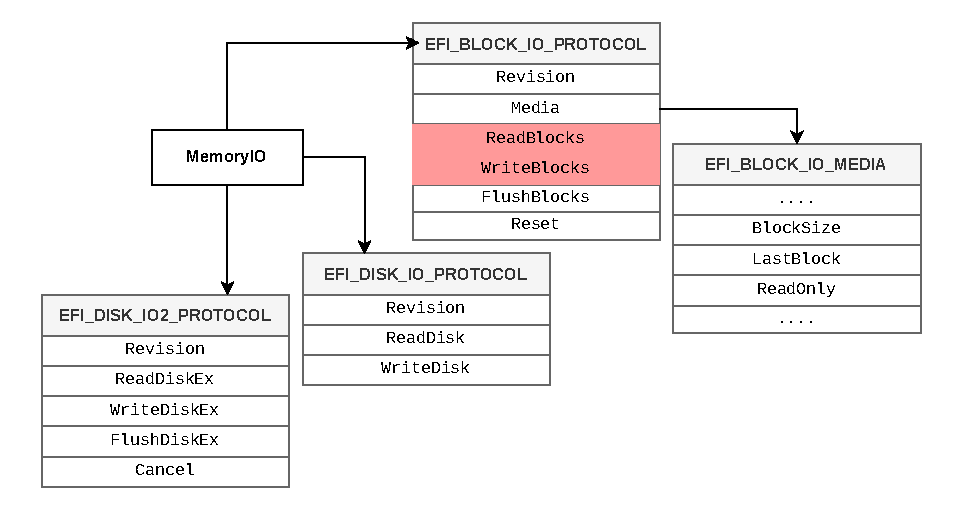
\includegraphics[width=0.8\textwidth]{MemoryIo.pdf} % Путь к файлу
	\caption{Интерфейсы, предоставляемые модулем MemoryIO.} % Подпись
	\label{env:pic:memoryio} % Метка для ссылок
\end{figure}

В реальной UEFI-среде драйверы файловых систем получают доступ к носителю через стандартизированные интерфейсы (см. рисунок \ref{env:pic:memoryio}):
\begin{itemize}
	\item\VarName{EFI\_BLOCK\_IO\_PROTOCOL} предоставляет доступ к блочному устройству, содержит информацию о носителе через \VarName{EFI\_BLOCK\_IO\_MEDIA}.\item\VarName{EFI\_DISK\_IO\_PROTOCOL} обеспечивает синхронный доступ к символьному устройству.\item\VarName{EFI\_DISK\_IO2\_PROTOCOL} расширяет \VarName{EFI\_DISK\_IO\_PROTOCOL}, добавляя поддержку асинхронных операций чтения/записи/сброса.
\end{itemize}
Полное описание можно найти в \cite{UEFISpec}.

Для эмуляции этих интерфейсов был разработан модуль\textbf{ MemoryIO}. Его основная задача  - <<создать>> в оперативной памяти виртуальное дисковое устройство на основе тестовых данных, передаваемых libFuzzer. Модуль возвращает структуру, содержащую полные реализации всех четырех требуемых интерфейсов.

Реализация функций в MemoryIO:
\begin{enumerate}
	\item \textbf{Синхронные операции (\FunName{ReadDisk}, \FunName{WriteDisk}) }эмулируются простым копированием данных из/в буфер, соответствующий виртуальному диску в памяти. Функции \FunName{FlushBlocks} и \FunName{Reset} реализованы как заглушки, так как физического устройства не существует.
	\item \textbf{Асинхронные операции  (\FunName{ReadDiskEx}, \FunName{WriteDiskEx}, \FunName{FlushDiskEx})}  эмулируют асинхронный ввод-вывод с использованием механизма событий UEFI:
	\begin{itemize}
		\item При вызове создается контекст задачи, содержащий тип операции, смещение, буфер данных и его размер.
		\item Создается  сигнальное событие \VarName{EFI\_EVENT}, с которым ассоциируется обработчик задачи и ее контекст.
		\item Создается однократный таймер EFI с небольшой задержкой (эмулирующей время выполнения операции). Этот таймер связывается с созданным событием.
		\item По истечении времени таймера срабатывает событие, вызывается обработчик, который выполняет запланированную операцию, сигнализирует о завершении операции и освобождает ресурсы задачи.
	\end{itemize}
	\item Функция \FunName{Cancel}  позволяет отменить все ожидающие асинхронные задачи.
    \item \textbf{Блочные функции (\FunName{ReadBlocks},\FunName{WriteBlocks})} не реализовывались, так как тестируемые драйверы не используют их напрямую.
\end{enumerate}

После инициализации MemoryIO возвращаемые им интерфейсы передаются тестируемому драйверу файловой системы. Драйвер использует их для монтирования виртуального диска и предоставления дескриптора корневого каталога \VarName{EFI\_FILE\_PROTOCOL}, через который осуществляются все операции с файловой системой.

\subsection{Эмуляция подсистемы событий UEFI Event}

Для обеспечения работы асинхронных операций и таймеров, задействованных как драйверами файловых систем, так и модулем MemoryIO, был реализован модуль \textbf{YummyEvent}. Он эмулирует ключевые функции подсистемы событий UEFI Boot Services \cite{UEFISpec}, включая:
\begin{itemize}
	 \item Создание/уничтожение событий \FunName{CreateEvent}/\FunName{CloseEvent}.
	 \item Сигнализация событий \FunName{SignalEvent}.
	 \item Ожидание событий \FunName{WaitForEvent}.
	 \item Управление таймерами \FunName{SetTimer}.
	 \item Контроль уровня привелегий \FunName{RaiseTPL}/\FunName{RestoreTPL}.
	 \item Проверка состояния событий \FunName{CheckEvent}.
	 \item Поддерживаемые типы событий: сигнальные, ожидающие, периодические таймеры.
\end{itemize}

Особенность реализации заключается в принципе явной диспетчеризации событий. Обработка событий (включая срабатывание таймеров и вызов callback-функций) не происходит в фоновых потоках. Вместо этого она инициируется исключительно при вызове методов UEFI Event, например таких как \FunName{SignalEvent}, \FunName{WaitForEvent} или \FunName{RaiseTPL}. Такой подход обеспечивает следующие характеристики:
\begin{itemize}
	\item Обработчики событий выполняются в контексте вполняющегося кода, что эмулирует поведение прерываний в UEFI среде.
	\item Отсутствие фоновой асинхронности гарантирует воспроизводимость результатов фаззинга.
	\item Упрощение отладки.
\end{itemize}

Для решения проблемы своевременного срабатывания таймеров введена функция \FunName{YummyEventsDispatch}. Её принудительный вызов позволяет <<продвинуть>> системное время, сработать ожидающим таймерам и обработать накопившиеся события. 

\section{Метод тестирования}

Разработанный метод фазинг-тестирования реализует комплексный подход, сочетающий синхронные и асинхронные сценарии для максимального покрытия функционала. Основу методики составляют шесть взаимодополняющих алгоритмов,

\textbf{FsFuzzSubTest1} выполняет работу с отдельным файлом: открытие на чтение, чтение метаданных файла, последовательное чтение блоков данных с перемещением позиции, а затем открытие на запись для записи данных в конец файла. Алгоритм выявляет ошибки управления файловыми дескрипторами, обработки позиционирования и операций ввода-вывода. Обобщенная схема работы алгоритма представлена на рисунке \ref{met:pic:fsfuzzsubtesti}.
\begin{figure}[htbp]
	\centering % Центрирование
	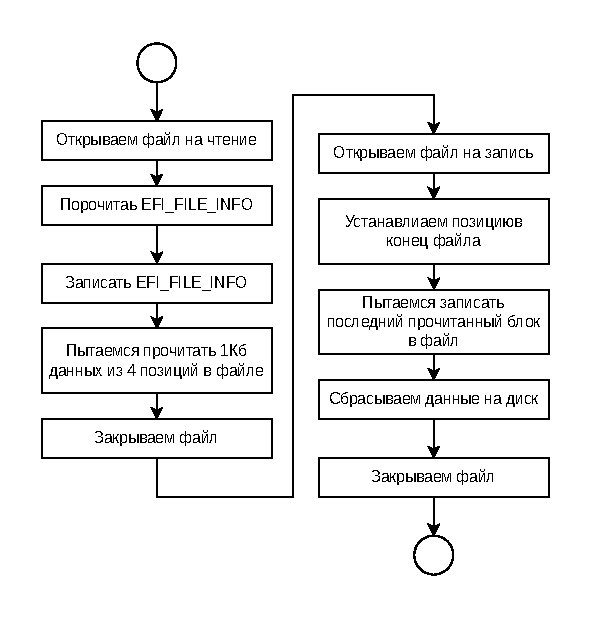
\includegraphics[width=0.5\textwidth]{FsFuzzSubtestI.pdf} % Путь к файлу
	\caption{Обобщенный алгоритм обработки файла \FunName{FsFuzzSubtest1}} % Подпись
	\label{met:pic:fsfuzzsubtesti} % Метка для ссылок
\end{figure}

\newpage
\textbf{FsFuzzTest1} реализует рекурсивный обход файловой системы с заданной глубиной. Для каждого обнаруженного файла он запускает \FunName{FsFuzzSubtest1}, а для катологов - рекурсивно углубляется в иерархию. Обобщенная схема алгоритма представлена на рисунке \ref{met:pic:fsfuzztesti}.
\begin{figure}[htbp]
	\centering % Центрирование
	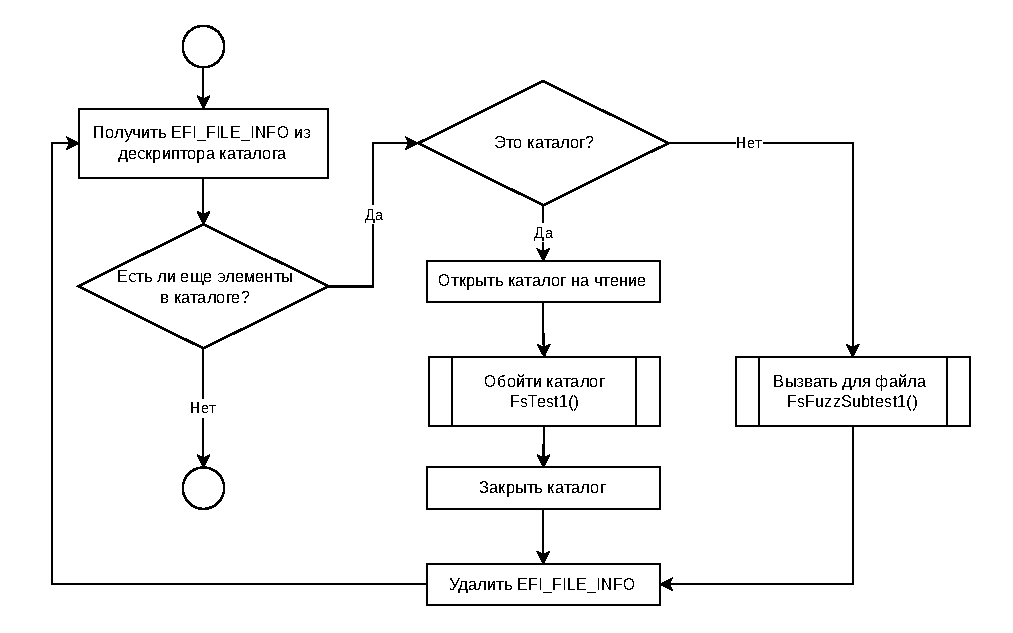
\includegraphics[width=0.7\textwidth]{FsFuzzTestI.pdf} % Путь к файлу
	\caption{Обобщенный алгоритм обхода каталога\FunName{FsFuzzTest1}} % Подпись
	\label{met:pic:fsfuzztesti} % Метка для ссылок
\end{figure}

\textbf{FsFuzzTest2} Последовательно открывает и удаляет все обычные файлы в текущем каталоге. Обобщенная схема алгоритма представлена на рисунке \ref{met:pic:fsfuzztestii}. 
\begin{figure}[htbp]
	\centering % Центрирование
	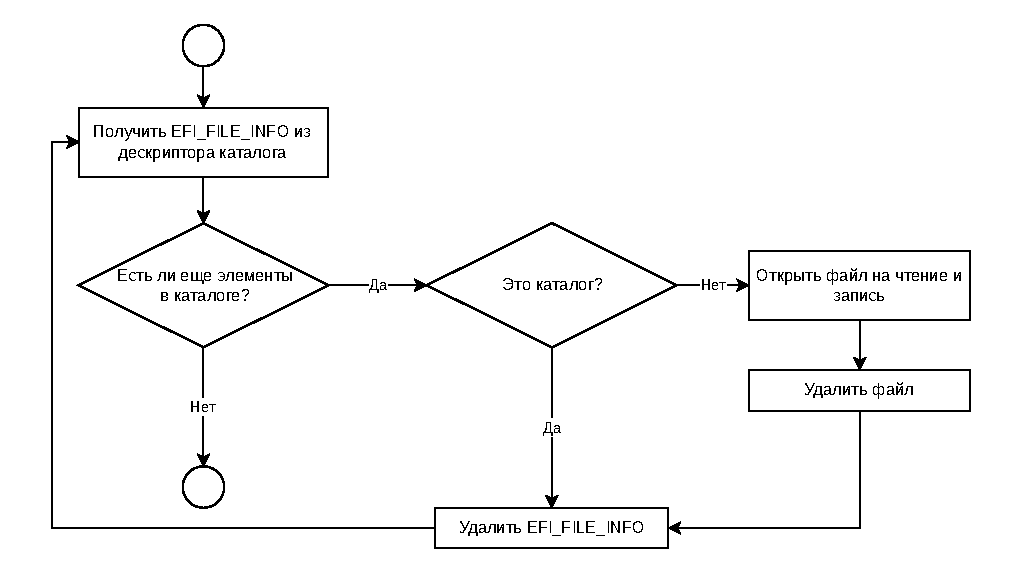
\includegraphics[width=0.7\textwidth]{FsFuzzTestII.pdf} % Путь к файлу
	\caption{Обобщенный алгоритм очистки каталога\FunName{FsFuzzTest2}} % Подпись
	\label{met:pic:fsfuzztestii} % Метка для ссылок
\end{figure}

\textbf{FsFuzzTest3} Создает цепочку вложенных директорий и файл на последнем уровне вложенности. Важно, что алгоритм создает файл, используя длинный путь к нему, но для успешного завершения этой операции необходимо создать все подпапки последовательно. Обобщенная схема алгоритма представлена на рисунке \ref{met:pic:fsfuzztestiii} 
\begin{figure}[h]
	\centering % Центрирование
	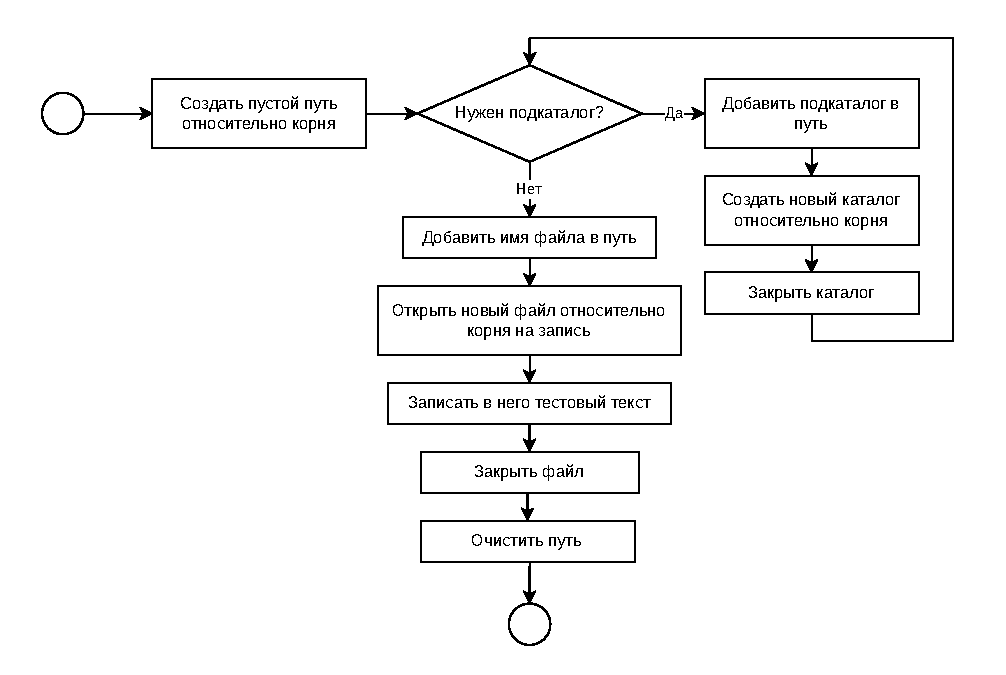
\includegraphics[width=0.7\textwidth]{FsFuzzTestIII.pdf} % Путь к файлу
	\caption{Обобщенный алгоритм создания тестового файла на длинном пути \FunName{FsFuzzTest3}} % Подпись
	\label{met:pic:fsfuzztestiii} % Метка для ссылок
\end{figure}

\textbf{FsFuzzAsyncWorker} - обработчик результата асинхронной задачи. После успешного открытия файла в асинхронном режиме планирует асинхронное чтение из этого файла. После успешного асинхронного чтения планирует асинхронную запись. После успешной асинхронной записи помечает асинхронную операцию выполненной, чтобы в дальнейшем освободить все занятые  задачей реурсы. Обобщенная схема алгоритма представлена на рисунке \ref{met:pic:fsfuzzasyncworker}.
\begin{figure}[h]
	\centering % Центрирование
	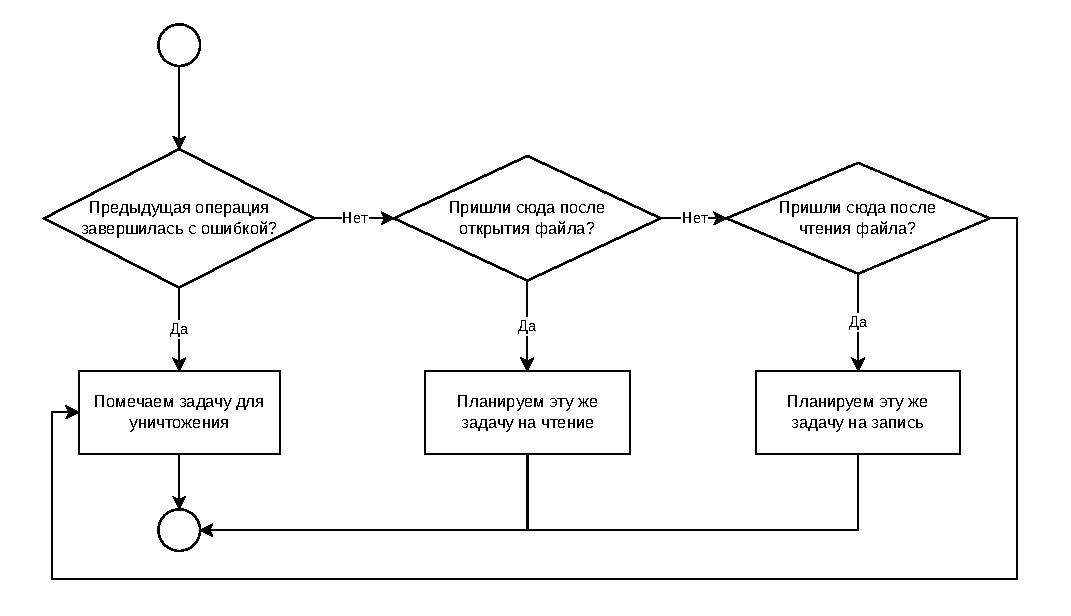
\includegraphics[width=0.7\textwidth]{FsFyzzAsyncWorker.pdf} % Путь к файлу
	\caption{Обобщенный алгоритм обработки асинхронной задачи \FunName{FsFuzzAsyncWorker}} % Подпись
	\label{met:pic:fsfuzzasyncworker} % Метка для ссылок
\end{figure}

\newpage
\textbf{FsFuzzTest4} дополняет асинхронную проверку, планируя параллельное выполнение операций \FunName{FsFuzzAsyncWorker} для всех файлов в каталоге. Обобщенная схема алгоритма представлена на рисунке \ref{met:pic:fsfuzztestiv}
\begin{figure}[htbp]
	\centering % Центрирование
	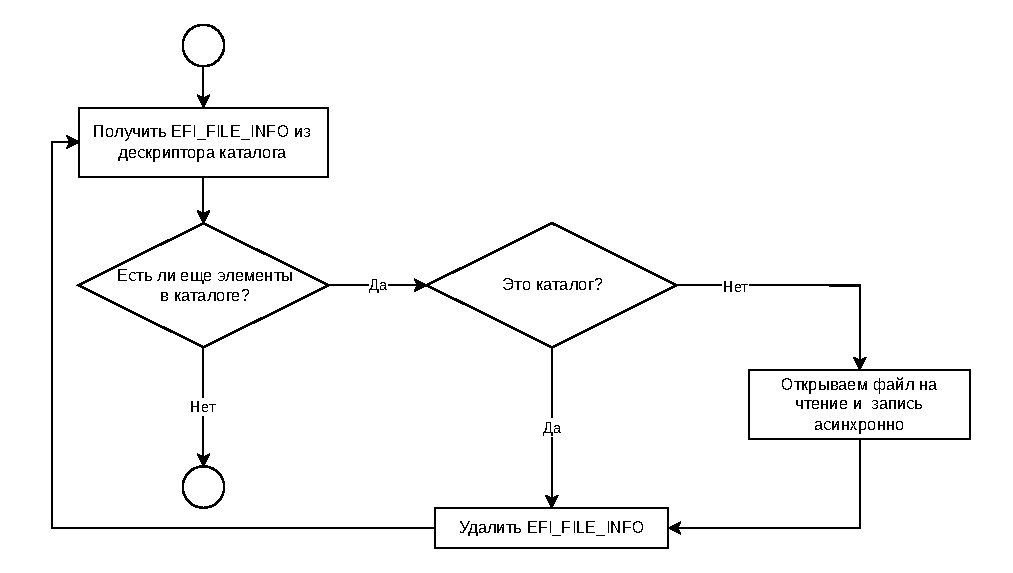
\includegraphics[width=0.7\textwidth]{FsFuzzIV.pdf} % Путь к файлу
	\caption{Обобщенный алгоритм планирования асинхронных операций над файлами из каталога \FunName{FsFuzzTest4}} % Подпись
	\label{met:pic:fsfuzztestiv} % Метка для ссылок
\end{figure}

Описанные сценарии тестирования используют стандартизированные функции из \VarName{EFI\_FILE\_PROTOCOL} и не вызывают каких-то узкоспециализированные функции драйвера напрямую. Это позволяет применять их для любых драйверов файловых систем, без необходимости дополнительного корректирования. Все сценарии последовательно вызываются из главной функции фаззинг-тестирования \FunName{FsFuzzTest}, которая принимает на вход только дескриптор корневого каталога. Алгоритм функции представлен на рисунке \ref{met:pic:fsfuzztest}.
\begin{figure}[htbp]
	\centering % Центрирование
	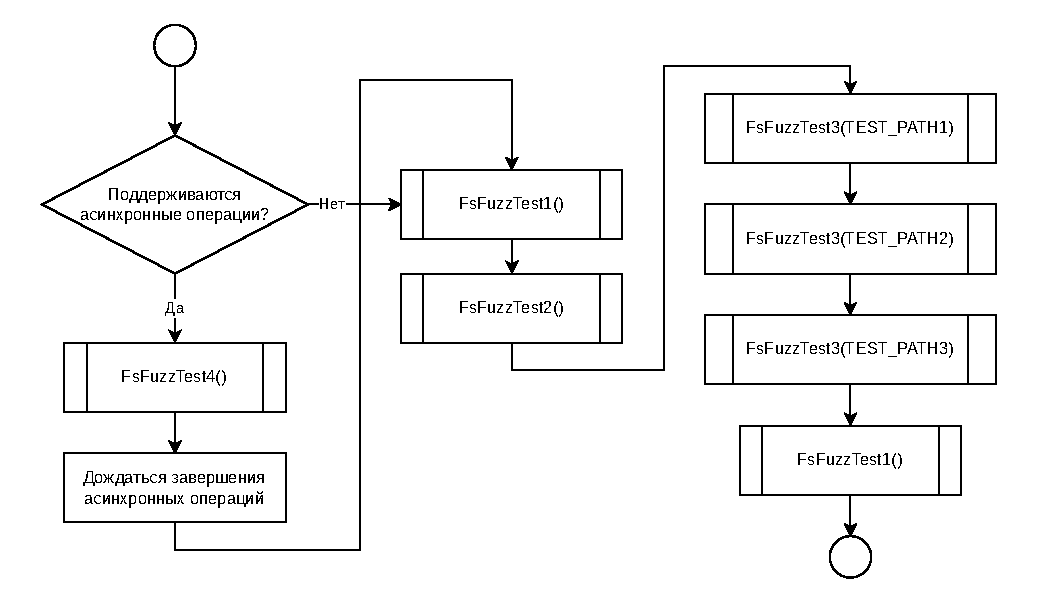
\includegraphics[width=0.75\textwidth]{FsFuzzTest.pdf} % Путь к файлу
	\caption{Главная функция, прводящая фаззинг-тестирование \FunName{FsFuzzTest}} % Подпись
	\label{met:pic:fsfuzztest} % Метка для ссылок
\end{figure} 

Все перечисленные функции поставляются модулем \textbf{FsFuzzTest}. В завершении на рисунке \ref{met:pic:testscheme} приведена обобщенная схема тестирования драйверов файловой системы, предложенная в этой работе  
\begin{figure}[htbp]
	\centering % Центрирование
	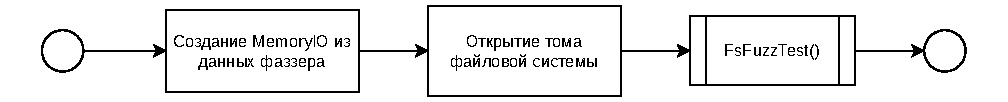
\includegraphics[width=0.8\textwidth]{TestScheme.pdf} % Путь к файлу
	\caption{Полная обобщенная схема предлагаемого метода фаззинг-тестирования} % Подпись
	\label{met:pic:testscheme} % Метка для ссылок
\end{figure} 
\section{Результаты тестирования драйвера FAT}

\subsection{Подготовка к тестированию}
Для запуска фаззинг-тестирования драйвера файловой системы FAT необходим начальный корпус из тестовых образов. Их генерация автоматизирована с помощью набора bash-скриптов (\textit{Test1.sh}-\textit{Test7.sh}). Скрипты создают образы, моделирующие разнообразные сценарии использования FAT.  Общая характеристика генерируемых образов:
\begin{itemize}
	\item Создаются образы FAT12, FAT16 и FAT32
	\item Различные размеры образов: от 8 Мб (маленькие образы для FAT12/FAT16) до 64 Мб (стандартный размер для FAT32)
	\item Используются разные размеры кластеров (512 байт и 2 Кб)
	\item Создается заданное количество папок (от 1 до 5) с файлами фиксированного (8 Кб) размера
	\item В корне размещаются файлы значительно большого размера (512 Кб, 2 Мб)
	\item Создаются цепочки вложенных папок (глубина от 2 до 3 уровней) с файлами на конечном уровне вложенности
	\item Большинство скриптов создает специальную папку FILLSPACE, которая заполняется по остаточному принципу до достижения заданного порога свободного места (1 Мб, 2 Мб, 8Мб) для имитации работы с почти заполненными образами
	\item Имена файлов и папок (длиной 32 символа) генерируются случайно из буквенно-цифрового набора. Скрипт \textit{Test7.sh} дополнительно включает имена с пробелами и специальными символами, проверяя корректность их обработки.
	\item Создаваемые файлы заполняются случайными данными из Linux-устройства \textit{/dev/urandom} 
\end{itemize} 
Такой подход к формированию начального корпуса позволяет эффективно тестировать базовые функции драйвера (чтение, запись, поиск, открытие/закрытие файлов и каталогов) в экстремальных и разнообразных условиях. Подробные параметры каждого скрипта сведены в таблице \ref{fat:tab:test_detail}.
\begin{table}[htbp]
	\renewcommand{\arraystretch}{1.5}
	\centering
	\begin{tabular}{|c|c|c|p{10cm}|}
		\hline
		\textbf{Скрипт} & \textbf{Размер} & \textbf{FAT} & \textbf{Описание} \\
		\hline
		\textit{Test1.sh} & 64 Мб & 32 &   4 корневые папки (по 10 файлов 8 Кб), 3 вложенные цепочки (глубина 3) с 10 файлами по 8 Кб на конце, 5 файлов в корне по  2Мб. FILLSPACE до 8 Мб. Размер кластера 512 байт \\
		\hline
		\textit{Test2.sh} & 32 Мб & 16 &   Структура идентична Test1 \\
		\hline
		\textit{Test3.sh} & 64 Мб & 16 &  Структура идентична Test2, но размер кластера увеличен до 2 Кб\\
		\hline
		\textit{Test4.sh} & 8 Мб & 12 &  2 корневые папки (по 5 файлов 8Кб), 1 вложенная цепочка (глубина 3) с 5 файлами по 8 Кб на конце,  3 файла в корне по 4 Кб. FILLSPACE до 2 Мб. Размер кластера 2 Кб \\
		\hline
		\textit{Test5.sh} & 64 Мб & 32 &  5 корневых папок (по 15 файлов 8 Кб), 4 вложенные цепочки (глубина 3) с 15 файлами по 8 Кб на конце, 2 файла  в корне по 2 МБ. Без заполнения FILLSPACE.  Размер кластера 2 Кб\\
		\hline
		\textit{Test6.sh} & 8 Мб & 16 &  Минималистичная структура: 1 корневая папка (3 файла), 1 вложенная цепочка (глубина 2, 3 файла), 2 файла по 512 КБ.  FILLSPACE до 1 Мб. Размер кластера 512 байт\\
		\hline
		\textit{Test7.sh} & 64 Мб & 32 & 3 корневые папки (по 5 файлов), 4 файла по 1 МБ, 2 вложенные цепочки (глубина 3, 3 файла). Имена с пробелами и спецсимволами. Без FILLSPACE. Размер кластера 512 байт  \\
		\hline
		
	\end{tabular}
	\caption{Подробные характеристики скриптов для создания образов}
	\label{fat:tab:test_detail}
\end{table}

Чтобы тестировать асинхронный функционал драйвера FAT, было отключено кеширование при вызове асинхронных функций, чтобы не ждать переполнение кеша, иначе операции все равно будут выполнены синхронно. Для этого в файле \FName{ReadWrite.c} драйвера были исправлены функции \FunName{FatReadEx} и \FunName{FatWriteEx} (см. листинг \ref{fat:listingA}): в вызов функции \FunName{FatIFileAccess} передаем флаги \FlagName{ReadDisk}/\FlagName{WriteDisk} вместо \FlagName{ReadData}/\FlagName{WriteData} 
\lstinputlisting[
caption={Файл \FName{ReadWrite.c}: изменения в функциях \FunName{FatReadEx} и \FunName{FatWriteEx}},
label={fat:listingA}
]{fatlistings/listingA.c} 

\subsection{Исправленные ошибки}

В процессе фаззинг-тестирования были обнаружены и исправлены следующие критические ошибки.

\begin{enumerate}
	\item \textbf{Неопределенное поведение (UB)} в функциях \FunName{FatGetDirEntInfo} и \FunName{FatOpenDirEnt} 
	
	\textbf{Файл} \FName{DirectoryManage.c}
	
	\textbf{Проблема:} При сборке номера кластера \VarName{Cluster} из 16-битных компонент сдвиг влево на 16 бит вызвал неявное приведение к типу \TypeName{int}, что привело к \ErrorName{UB} при переполнении \cite{ISO_C17}
	
	\textbf{Исправление:} Явное приведение к \TypeName{UINTN} (см. листинги \ref{fat:listingB} и \ref{fat:listingC})
	\lstinputlisting[
	caption={Файл \FName{DirectoryManage.c}, кусок кода функции \FunName{FatGetDirEntInfo}:  BEFORE - до исправления, AFTER - после исправления},
	label={fat:listingB}
	]{fatlistings/listingB.c} 
	\lstinputlisting[
	caption={Файл \FName{DirectoryManage.c}, кусок кода функции \FunName{FatOpenDirEnt}:  BEFORE - до исправления, AFTER - после исправления},
	label={fat:listingC}
	]{fatlistings/listingC.c} 
	
	\item \textbf{Утечка памяти (MemoryLeak) и взаимоблокировка (DeadLock)} в функции \FunName{FatIFileAccess}
	
	\textbf{Файл:} \FName{ReadWrite.c}
	
	\textbf{MemoryLeak:} При ошибке в \FunName{FatGrowEof} не освобождается объект асинхронной задачи
	
	\textbf{DeadLock:} Блокировка тома не снималась перед вызовом \FunName{FatQueueTask}, что может вызвать взаимоблокировку при обработке связанного с задачей сигнала
	
	\textbf{Исправление:}
	\begin{itemize}
		\item Добавлено освобождение задачи при ошибках (строки 9-11 листинга \ref{fat:listingD})
		\item Снятие блокировки тома перед \FunName{FatQueueTask} и при ошибках (строки 13 и 19 листинга  \ref{fat:listingD})
	\end{itemize}
	\lstinputlisting[
	caption={Файл \FName{ReadWrite.c}, кусок кода функции \FunName{FatIFileAccess}:  комментариями отмечены типы исправленных ошибок},
	label={fat:listingD}
	]{fatlistings/listingD.c} 
	
	\item \textbf{Доступ после освобождения (UseAfterFree)} в \FunName{FatQueueTask}
	
	\textbf{Файл:} \FName{Misc.c}
	
	\textbf{Проблема:} Итерация по списку подзадач без блокировок приводила к доступу к освобождённой памяти, если элементы удалялись в обработчике событий
	
	\textbf{Исправление:} Добавлены блокировки \VarName{FatTaskLock} во время итераций по списку (см. листинг \ref{fat:listingE})
	\lstinputlisting[
	caption={Файл \FName{Misc.c}:  переписанная функция \FunName{FatQueueTask}, многоточиями отмечены похожие с предыдущей версией места},
	label={fat:listingE}
	]{fatlistings/listingE.c} 
	
\end{enumerate}

\newpage
Итоговое количество обнаруженных и исправленных на данный момент ошибок сведено в таблице \ref{fat:tab:sumerror}.
\begin{table}[htbp]
	\renewcommand{\arraystretch}{1.5}
	\centering
	\begin{tabular}{|c|c|}
		\hline
		\textbf{Тип} & \textbf{Количество} \\
		\hline
		\ErrorName{UB} & 2 \\
		\hline
		\ErrorName{MemoryLeak} & 1 \\
		\hline
		\ErrorName{DeadLock} & 1 \\
		\hline
		\ErrorName{UseAfterFree} & 1 \\
		\hline
	\end{tabular}
	\caption{Тип и количество исправленных ошибок в драйвере FAT}
	\label{fat:tab:sumerror}
\end{table}

\subsection{Покрытие кода}
Результирующее покрытие кода драйвера FAT сведено в таблице \ref{fat:tab:coverage}
\begin{table}[ht]
	\centering
	\begin{tabular}{|c|c|c|c|}
		\hline
		\textbf{Filename} & \textbf{Line} & \textbf{Branch} & \textbf{Function} \\
		\hline
		\FName{Delete.c}&  58.3\% &  32.4\% &  100.0\% \\
		\FName{DirectoryCache.c} &  100.0\% &  70.6\% &  100.0\% \\
		\FName{DirectoryManage.c} &  76.7\% &  62.9\% &  80.8\% \\
		\FName{DiskCache.c} &  80.1\% &  76.6\% &  85.7\% \\
		\FName{FileName.c} &  89.1\% &  86.7\% &  100.0\% \\
		\FName{FileSpace.c} &  88.0\% &  79.0\% &  91.7\% \\
		\FName{Flush.c} &  86.6\% &  70.2\% &  100.0\% \\
		\FName{Hash.c} &  100.0\% &  100.0\% &  100.0\% \\
		\FName{Info.c} &  37.6\% &  30.4\% &  55.6\% \\
		\FName{Init.c} &  73.3\% &  51.1\% &  66.7\% \\
		\FName{Misc.c} &  87.2\% &  62.8\% &  94.1\% \\
		\FName{Open.c} &  85.4\% &  72.9\% &  100.0\% \\
		\FName{OpenVolume.c} &  84.6\% &  50.0\% &  100.0\% \\
		\FName{ReadWrite.c} &  87.3\% &  69.4\% &  100.0\% \\
		\FName{UnicodeCollation.c} &  47.4\% &  0.0\% &  71.4\% \\
		\hline
	\end{tabular}
	\caption{Покрытие кода драйвера FAT}
	\label{fat:tab:coverage}
\end{table}
\section{Результаты тестирования драйвера ext4}

\subsection{Подготовка к тестированию}
Для тестирования драйвера файловой системы ext4 были разработаны bash-скрипты (\textit{Test1.sh}-\textit{Test10.sh}), которые автоматизируют создание тестовых образов для начального корпуса. Подробное описание каждого скрипта приведено в таблице \ref{ext:tab:test_detail}. Основные характеристики генерируемых образов:
\begin{itemize}
	\item Многоуровневые вложенные директории (до 8 уровней).
	\item Различные типы ссылок (символические и жесткие).
	\item Специальные случаи: ссылки на себя, родительские и корневые директории.
	\item Ссылки за пределы образа.
	\item Жесткие ссылки на один inode.
	\item Отдельный тест создает длинные имена (200-255 символов).
	\item Заполнение образа до заданного порога свободного места при помощи папки FILLSPACE.
	\item Различные размеры файов (от 1 Кб до 2 Мб).
	\item Создание некорректных симлинков.
	\item Все скрипты создают образ рахмером в 64 Мб.
\end{itemize} 
\begin{table}[htbp]
	\renewcommand{\arraystretch}{1.5}
	\centering
	\begin{tabular}{|c|p{10cm}|}
		\hline
		\textbf{Скрипт} & \textbf{Описание} \\
		\hline
		\textit{Test1.sh} & Базовая структура: 4 корневые папки (по 10 файлов), 3 вложенные цепочки (глубина 3), 5 файлов по 2 МБ в корне.\\
        \hline
        \textit{Test2.sh} & Структура Test1 + символические ссылки в корне на поддиректории уровня 2.\\
        \hline
        \textit{Test3.sh} & 1 папка (10 файлов) + символическая ссылка на себя внутри папки + символическая ссылка на папку в корне + 5 файлов по 2 МБ.\\
        \hline
        \textit{Test4.sh} & Структура Test3 + символическая ссылка на корневую директорию внутри папки. \\
        \hline
        \textit{Test5.sh} & Структура Test4 + символическая ссылка на внешнюю папку за пределами образа. \\
        \hline
        \textit{Test6.sh} & Глубокая вложенность (8 уровней) + файлы на каждом уровне + символические ссылки на предыдущий уровень и корень (за пределы образа). \\
        \hline
        \textit{Test8.sh} & Создание: 50 папок (по 100 файлов по 1K) + символические ссылки между папками $(i\rightarrow i+10)$, где $i=1...10$. Заполнение FILLSPACE отсутствует.\\
        \hline
        \textit{Test9.sh} & Жесткие ссылки: 1 исходный файл + 15 жестких ссылок (10 в корне, 5 в подпапке) + 1 несвязанный файл.\\
        \hline
        \textit{Test10.sh} & Длинные имена (200-255 символов): директория + 5 файлов + символическая ссылка на директорию в корне + файл в корне.\\
        \hline
	\end{tabular}
	\caption{Подробные характеристики скриптов для создания образов.}
	\label{ext:tab:test_detail}
\end{table}

\newpage
\subsection{Исправленные ошибки}
\begin{enumerate}
	\item \textbf{Не следование спецификации}.
	
	\textbf{Файл:} \FName{Partition.c}.
	
	\textbf{Проблема:} Драйвер не поставляет функцию \FunName{Flush}, хотя по спецификации она обязана присутствовать \cite{UEFISpec}.
	
	\textbf{Решение:} Так как драйвер ReadOnly, то реализована заглушка  \FunName{\_Ext4Flush} (см. листинг \ref{ext:listingA}) и заполняется поле \VarName{Flush} файлового протокола в функции \FunName{Ext4SetupFile} (см. листинг \ref{ext:listingB}).
	\lstinputlisting[
	caption={Файл \FName{Partition.c}: функция-заглушка \FunName{\_Ext4Flush}},
	label={ext:listingA}
	]{extlistings/listingA.c} 
	\lstinputlisting[
	caption={Файл \FName{Partition.c}, кусок кода функции \FunName{Ext4Setup}: установка заглушки.},
	label={ext:listingB}
	]{extlistings/listingB.c} 
	
	\item \textbf{Раскрытие ASSERT} в функции \FunName{Ext4ReadFile}.
	
	\textbf{Файл:} \FName{File.c}.
	
	\textbf{Проблема:} Срабатывание \FunName{ASSERT}.
	
	\textbf{Решение:} Заменить \FunName{ASSERT} на явную обработку ошибки (листинг \ref{ext:listingC}).
	 \lstinputlisting[
	 caption={Файл \FName{File.c}, кусок кода функции \FunName{Ext4ReadFile}: явная обработка \FunName{ASSERT}.},
	 label={ext:listingC}
	 ]{extlistings/listingC.c} 
\end{enumerate}

Итоговое количество обнаруженных и исправленных на данный момент ошибок сведено в таблице \ref{ext:tab:sumerror}.
\begin{table}[htbp]
	\renewcommand{\arraystretch}{1.5}
	\centering
	\begin{tabular}{|c|c|}
		\hline
		\textbf{Тип} & \textbf{Количество} \\
		\hline
		Не следование спецификации & 1 \\
		\hline
		\ErrorName{Assert} & 1 \\
		\hline
	\end{tabular}
	\caption{Тип и количество исправленных ошибок в драйвере ext4.}
	\label{ext:tab:sumerror}
\end{table}

\newpage
\subsection{Покрытие кода}
Результирующее покрытие кода драйвера ext4 сведено в таблице \ref{ext:tab:coverage}.
\begin{table}[ht]
	\centering
	\begin{tabular}{|c|c|c|c|}
		\hline
		\textbf{Filename} & \textbf{Line} & \textbf{Branch} & \textbf{Function} \\
		\hline
\FName{BlockGroup.c} & 75.0\% & 54.5\% & 83.3\% \\
\FName{BlockMap.c} & 0.0\% & 0.0\% & 0.0\% \\
\FName{Directory.c} & 87.3\% & 80.4\% & 100.0\% \\
\FName{DiskUtil.c} & 73.1\% & 50.0\% & 100.0\% \\
\FName{Ext4Dxe.c} & 0.0\% & 0.0\% & 0.0\% \\
\FName{Extents.c} & 48.5\% & 36.5\% & 73.3\% \\
\FName{File.c} & 66.8\% & 62.9\% & 85.0\% \\
\FName{Inode.c} & 88.5\% & 59.5\% & 100.0\% \\
\FName{Partition.c} & 90.0\% & 66.7\% & 100.0\% \\
\FName{Superblock.c} & 66.0\% & 55.7\% & 83.3\% \\
\FName{Symlink.c} & 66.7\% & 59.4\% & 100.0\% \\
		\hline
	\end{tabular}
	\caption{Покрытие кода драйвера ext4.}
	\label{ext:tab:coverage}
\end{table}

\section{Результаты тестирования драйвера EFI NTFS}

\subsection{Подготовка к тестированию}
Аналогично FAT и ext4 был разработан набор bash-скриптов (\textit{Test1.sh}-\textit{Test8.sh}), создающих специализированные тестовые образы файловой системы NTFS, которые составят начальный корпус для фаззинг-тестирования. Эти скрипты охватывают ключевые особенности NTFS, включая поддержку различных размеров кластеров, работу с метаданными, обработку сложных структур ссылок и экстремальных случаев. Подробные характеристики приведены в таблице \ref{ntfs:tab:test_detail}. Основные характеристики генерируемых образов:
\begin{itemize}
	\item Многоуровневые вложенные директории (до 4 уровней).
	\item Различные типы ссылок (символические и жесткие).
	\item Специальные случаи (ссылки на себя, корневые директории, за пределы образа).
	\item Различные размеры кластеров.
	\item Различные размеры образов (8 Мб - 32 Мб).
	\item Аналогичное заполнение до указанного порога (FILLSPACE, только Test1.sh).
	\item Генерация как стандартных, так и длинных имен со специальными символами.
	\item Жесткие ссылки на один файл.
\end{itemize} 

\begin{table}[htbp]
	\renewcommand{\arraystretch}{1.5}
	\centering
	\begin{tabular}{|c|c|p{10cm}|}
		\hline
		\textbf{Скрипт} & \textbf{Размер} & \textbf{Описание} \\
		\hline
		\textit{Test1.sh} & 16 Мб & Базовая структура: 4 корневые папки (по 10 файлов), 3 вложенные цепочки (глубина 3), 3 файла по 2 Мб в корне. FILLSPACE до 2 Мб. \\
		\hline
		\textit{Test2.sh} & 32 Мб & Нестандартный размер кластера (8 Кб). 5 корневых папок (по 15 файлов), 4 вложенные цепочки (глубина 4), 10 файлов по 1 Мб.\\
		\hline
		\textit{Test3.sh} & 32 Мб &Длинные имена (200 символов) со спецсимволами. 20 папок (по 200 файлов по 1 Кб) + символические ссылки на себя и из корня. \\
		\hline
		\textit{Test4.sh} & 8 Мб & Маленький образ. 20 папок (по 10 файлов по 1 Кб) + символические ссылки на себя в каждой папке и из корня на папки.\\
		\hline
		\textit{Test5.sh} & 16 Мб & Жесткие ссылки: 1 базовый файл (2 Мб) + 10 ссылок в корне + 5 ссылок в подпапке.\\
		\hline
		\textit{Test6.sh} & 16 Мб & Массовое создание файлов: 10 папок × 500 файлов (всего 5000). \\
		\hline
		\textit{Test7.sh} & 16 Мб & Папки с символическими ссылками: 5 папок (по 10 файлов), в каждой символические ссылки на себя и на корневую директорию.\\
		\hline
		\textit{Test8.sh} & 16 Мб & Символическая ссылка на внешнюю директорию: 5 папок (по 10 файлов), в каждой символические ссылки на себя, корень и внешнюю папку за пределами образа.\\
		\hline
	\end{tabular}
		\caption{Подробные характеристики скриптов для создания образов.}
	\label{ntfs:tab:test_detail}
\end{table}

\newpage
\subsection{Ошибки, обнаруженные при тестировании}
\begin{enumerate}
	\item \textbf{Не следование спецификации.}
	
	\textbf{Файл:} \FName{NTFS.c}.
	
	\textbf{Проблема:} В функции \FunName{NTFSStart} указывается некорректная версия файлового протокола (см. листинг \ref{ntfs:listingA}), вторая версия файлового протокола требует наличия асинхронных функций, которые драйвер не поставляет \cite{UEFISpec}.
    
    \textbf{Решение:} Указать правильный номер версии.
	\lstinputlisting[
	caption={Файл \FName{NTFS.c}, кусок кода функции \FunName{NTFSStart}: некорректная версия файлового протокола},
	label={ntfs:listingA}
	]{ntfslistings/listingA.c} 
	
	\item \textbf{Не возвращается признак конца каталога}.
	
	\textbf{Файл:} \FName{Open.c}.
	
	\textbf{Проблема:} Функция \FunName{FileRead} не возвращает признак конца каталога, как того требует спецификация \cite{UEFISpec}.
	
	\textbf{Текущий статус:} Не решена.
\end{enumerate}

\subsection{Покрытие кода}
На момент сдачи работы измерение покрытия кода для драйвера EFI NTFS \textbf{невозможно} из-за критической ошибки, приводящей к зависанию тестов при работе с каталогами. Для получения валиндных метрик необходимо исправить эту ошибку. 
\section{Заключение}
В ходе выполнения курсовой работы разработан метод фаззинг-тестирования драйверов файловых систем в UEFI-окружении. Основные результаты включают:
\begin{enumerate}
	\item Доработку пользовательского окружения подсистемой событий UEFI Event.
	\item Реализацию шести тестовых сценариев, охватывающих синхронные и асинхронные операции с файлами и каталогами через стандартизированный интерфейс \VarName{EFI\_FILE\_PROTOCOL}.
	\item Автоматизированную генерацию начальных корпусов из образов тестируемых файловых систем.
	\item Обнаружение и исправление ошибок в драйверах.
	\item Получение метрик покрытия кода для драйверов FAT и ext4.
\end{enumerate}

В продолжении этой работы планируется:
\begin{itemize}
	\item Продолжение фаззинг-тестирования драйверов FAT, ext4 и EFI NTFS с исправлением выявленных ошибок.
	\item Оптимизация используемых сценариев, подбор оптимальных параметров, чтобы ускорить тестирование.
	\item Исследовать сценарий, при котором синхронные операции не дожидаются завершения асинхронных.
	\item Исследование ресурсоемкости метода. Даже несмотря на использование различных типов аллокаторов экспоненциально растет потребление памяти, что не дает запустить фаззер на долгое время. Возможно требуется провести исследование потребления памяти у используемого окружения.
\end{itemize} 

% СПИСОК ЛИТЕРАТУРЫ
\bibliographystyle{gost71u}
\bibliography{references}

\end{document}